\section{Tuning}\label{sec:tuning}

The initial parameters, based on the sampling time and expected 
noise of the sensor and the sampling time, provided a good starting point.
What was lacking appeared to be an ability of the system to make proper turns.
A possible explanation is that the calculated noises dont account for
any significant maneuvering. 
The noises should therefore be slightly increased in order for the filter
to also account for reasonable changes in attitude and position.
When tuning the simulated data, the initial tuning was done roughly like this:
Tune measurement noise until the GNSS track is followed.
Tune process noise to get a decent NEES results.
Tune IMU bias driving noises to reduce trends in gyro and acceleration NEES bias.
Tune individual measurement and process noise parameters to fit individual IMU NEES axis.

An observation made was that certain larger deviations occured in the NEESes. 
This appears to be due to larger then normal changes in position and attitude. 
Due to the infrequent GNSS updates, the process noise was increased while
the measurement noises was decreased to try to better account for these occurrences.
The reasoning being that the IMU might be able track the true value better.
Reducing measurement noise in favour of process noise also improved NIS results, 
by reducing overfitting in parts of the track.

The tuning appeared in large part to be a bias-variance tradeoff problem.
Our experience was that reducing the variance during large state changes led to overfitting elsewhere.
From a practical point of view we would argue that it makes more sense to track the large state changes better
and accept some overfitting elsewhere if the alternative is to have huge errors in certain parts of the track.
This is of course a tradeoff and also there are probably situations where an opposite argument could be made.

\begin{tabular}{ |p{5cm}||p{2cm}|p{2cm}|  }
	\hline
	\multicolumn{3}{|c|}{Results} \\
	\hline
	Parameter & Sim. data & Real data\\
	\hline
	NIS mean			& 1.4971  	&   0.9940\\
	NEES tot mean		& 13.0695 	&	-\\
	NEES pos mean 		& 1.4101 	&  -\\
	NEES vel mean		& 0.9584 	& -\\
	NEES att mean		& 0.9281 	& -\\
	NEES acc bias mean	& 5.3252 	& -\\
	NEES gyr bias mean 	& 0.9258 	& -\\
	Est pos RMSE		& 0.5637 	& -\\
	Est vel RMSE		& 0.3485 	& -\\
	Meas pos RMSE		& 0.6735 	& -\\
	\hline
\end{tabular}

\begin{tabular}{ |p{5.5cm}||p{4cm}|p{4cm}|  }
	\hline
	\multicolumn{3}{|c|}{Tuned parameters} \\
	\hline
	Parameter & Simulated data & Real data\\
	\hline
	Rate std.			& 2.6160e-5 sqrt(1/dt)	&   4.36e-5 sqrt(1/dt)\\
	Acc std.			& 7.5855e-3	sqrt(1/dt)  &	0.9336e-3 sqrt(1/dt)\\
	Cont rate bias driving noise std	& 3e-3 sqrt(1/dt)	& 5e-5 / np.sqrt(1/dt)\\	
	Cont acc bias driving noise std		& 24e-4 sqrt(1/dt)	& 4e-3 / np.sqrt(1/dt)\\
	p std.							& [0.4, 0.5, 0.6]**2 	& [0.2, 0.2, 0.4]**2\\
	p acc							& 1e-6 		& 1e-12\\
	p gyro 							& 1e-4 		& 1e-12\\
	\hline
\end{tabular}

\begin{figure}
    \centering
    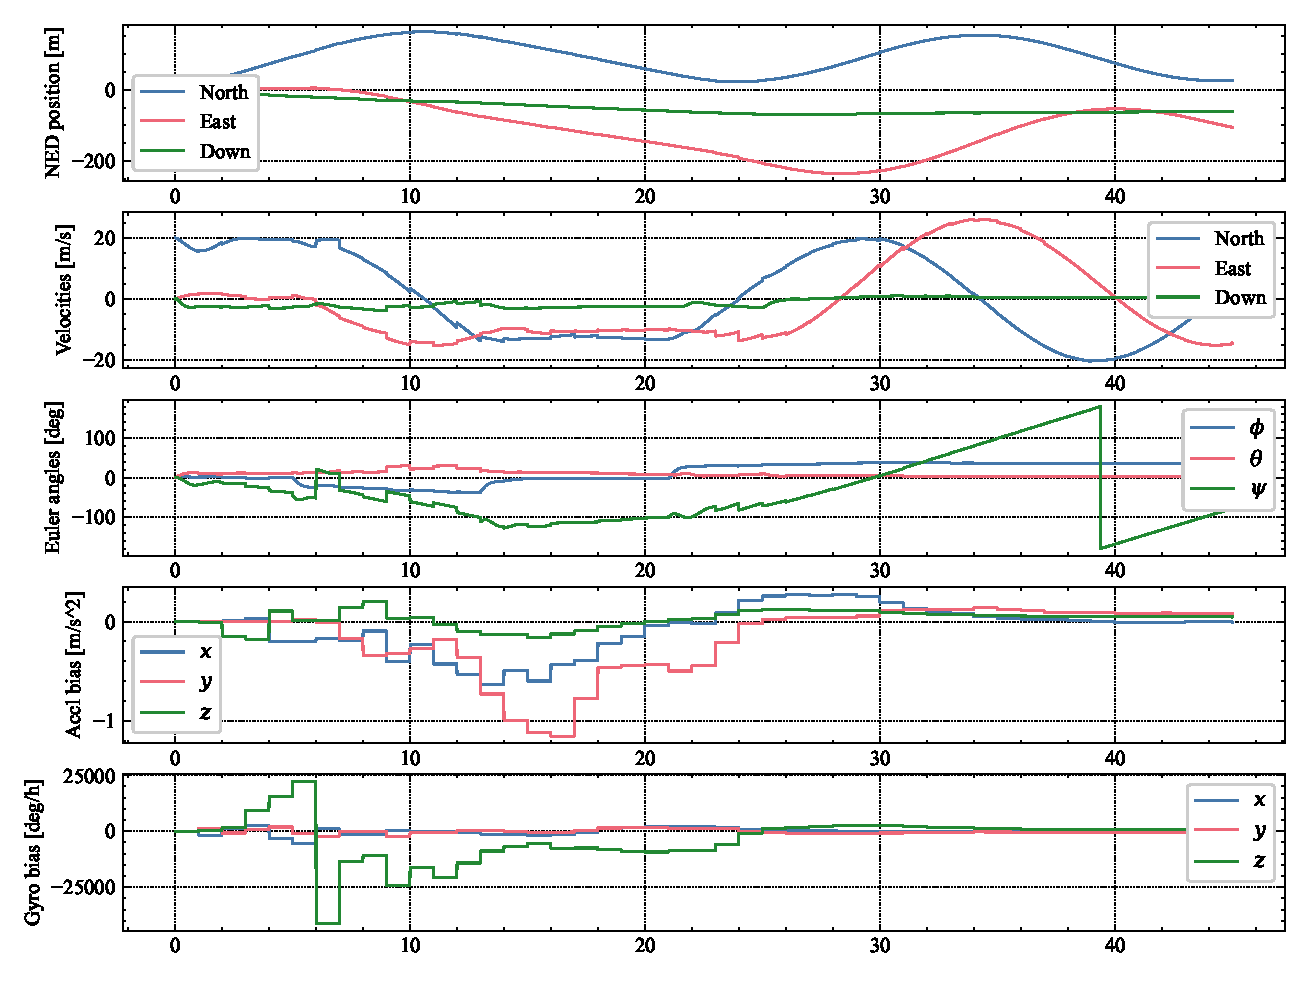
\includegraphics[clip, trim= 0cm 0cm 0cm 0cm, width = \textwidth]{figures/sim_2.eps}
    \caption{Estimated states}
	\label{fig:1_2}
	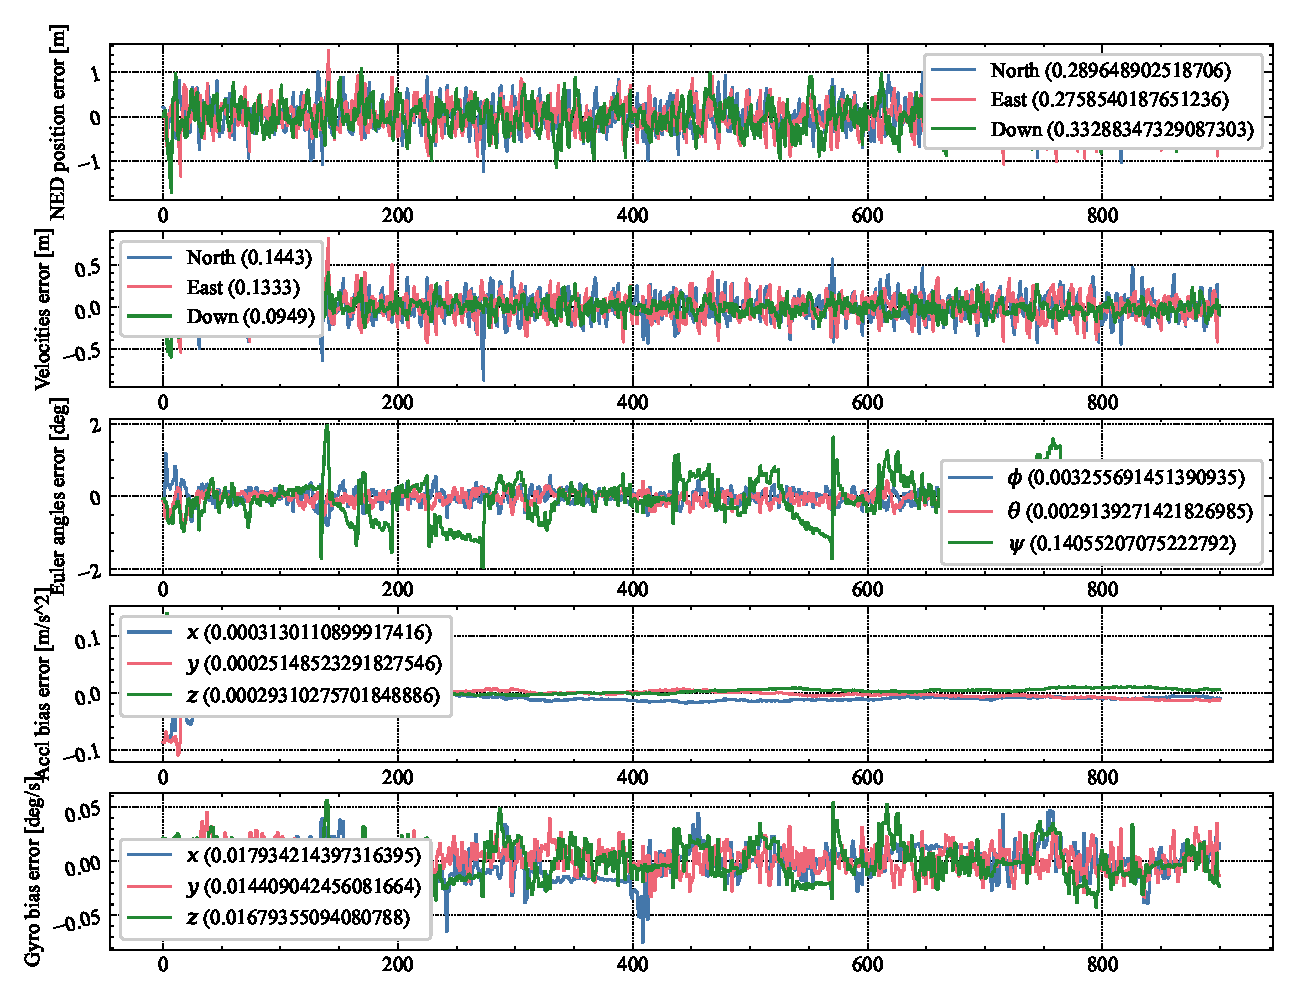
\includegraphics[clip, trim= 0cm 0cm 0cm 0cm, width = \textwidth]{figures/sim_3.eps}
    \caption{True error states}
	\label{fig:23states}
\end{figure}
\begin{figure}
	\centering
	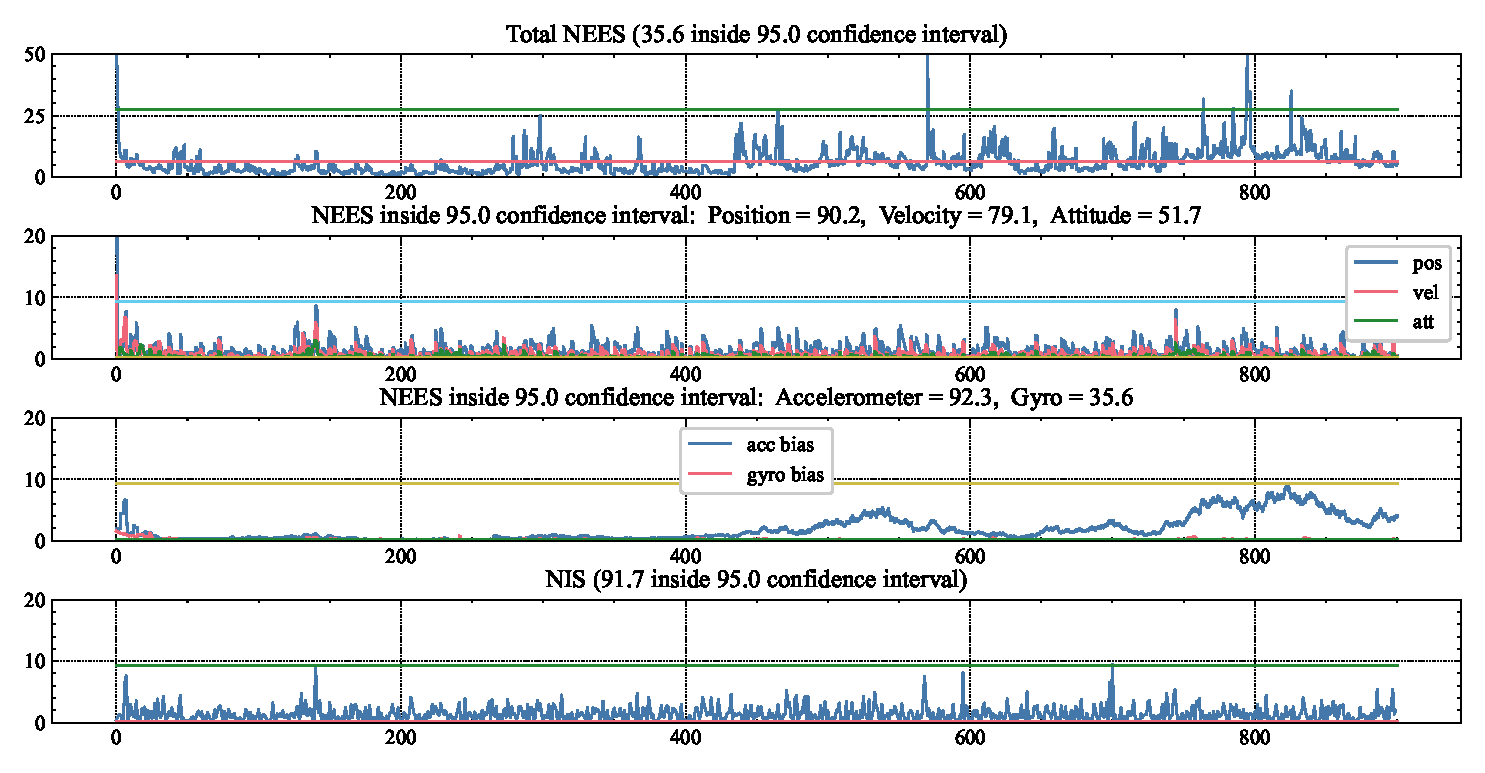
\includegraphics[clip, trim= 0cm 0cm 0cm 0cm, width = \textwidth]{figures/sim_10.eps}
    \caption{NEESes and NIS}
    \label{fig:23states}
    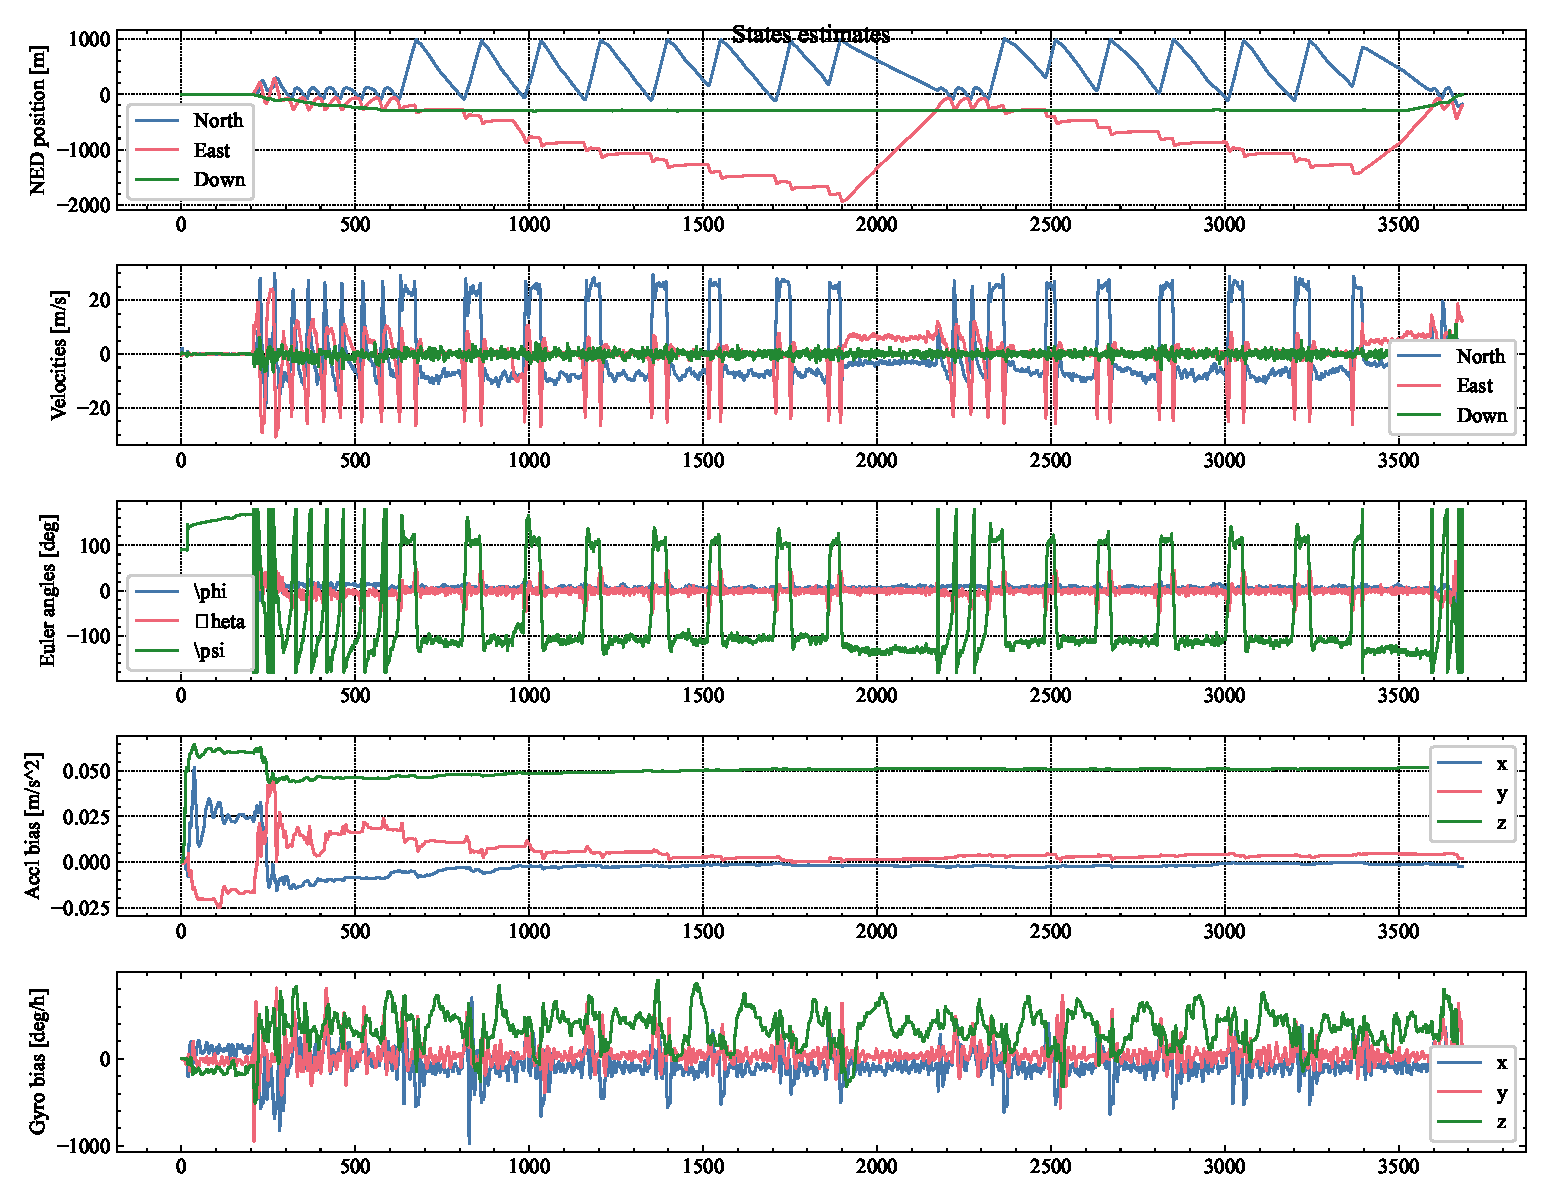
\includegraphics[clip, trim= 0cm 0cm 0cm 0cm, width = \textwidth]{figures/real_2.eps}
    \caption{True error states}
	\label{fig:23states}
	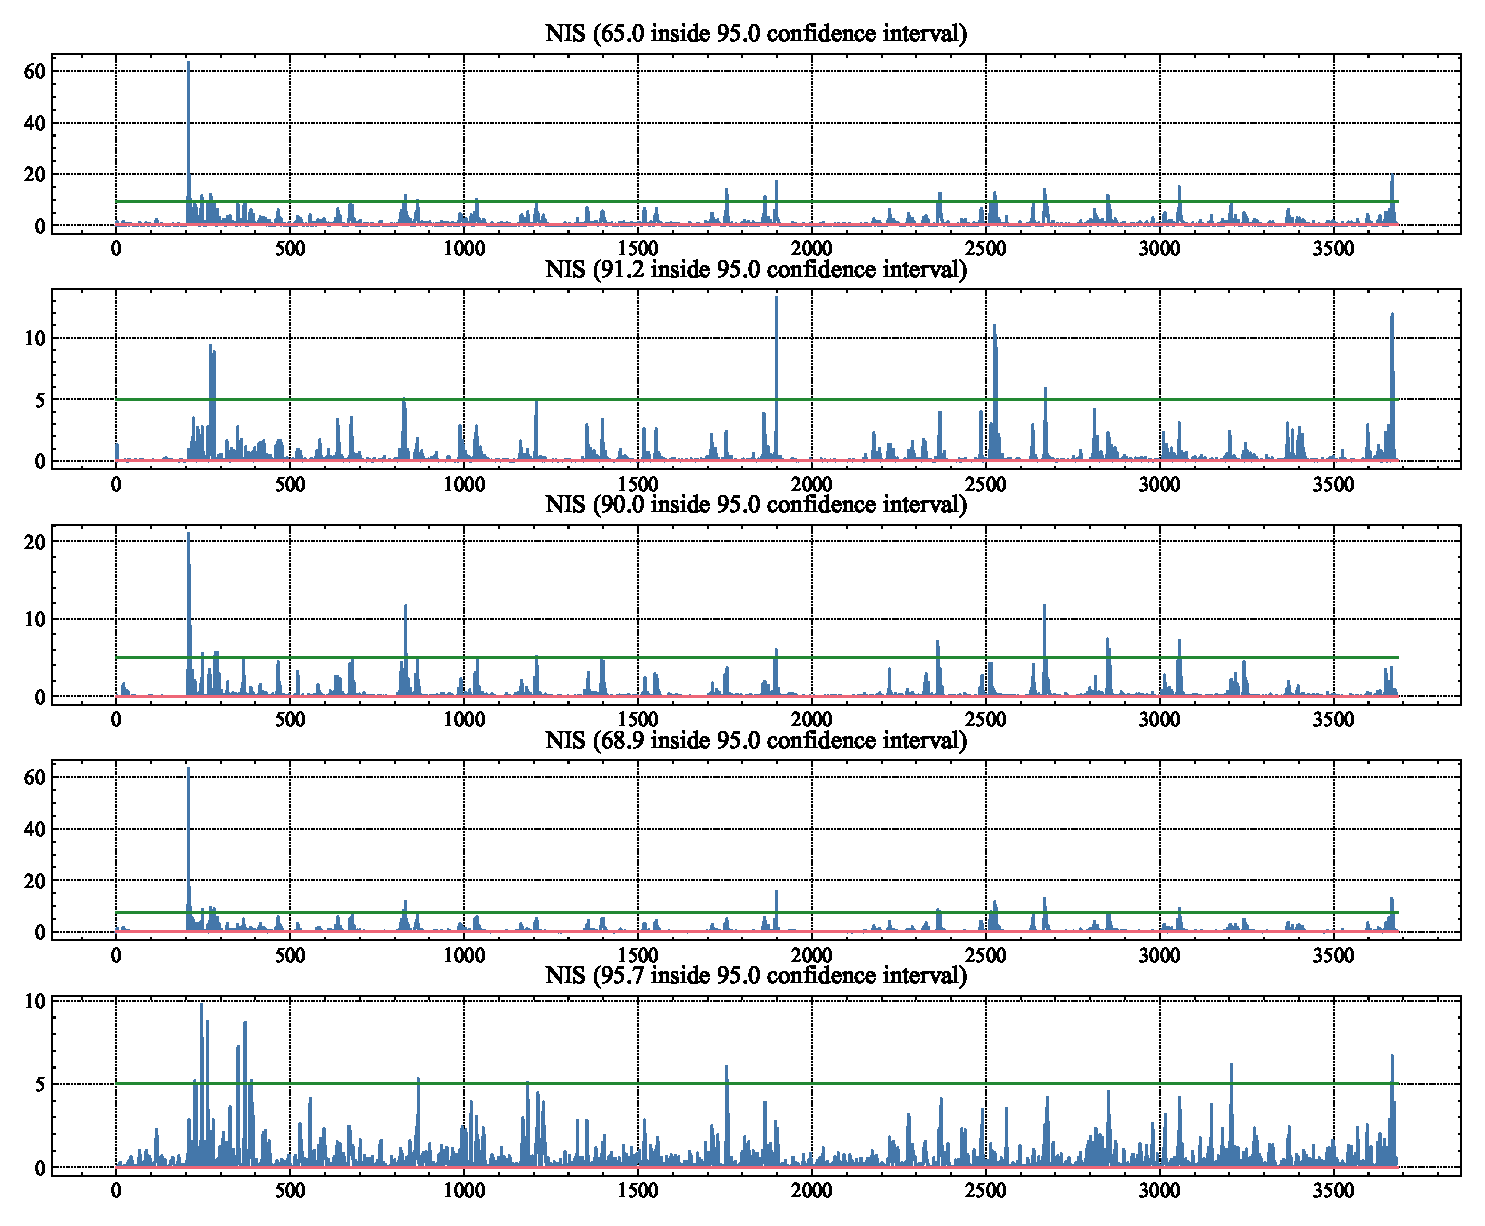
\includegraphics[clip, trim= 0cm 0cm 0cm 0cm, width = \textwidth]{figures/real_3.eps}
    \caption{NEESes and NIS}
    \label{fig:23states}
\end{figure}

\subsection*{Task 3b}

The heading is observable during motion due to the GNSS updates. The degree of observability depends
on the type of motion, and when coming to a stop the heading would no longer be observable due to GNSS.
However the IMU would still allow the heading to be observable although colored noise would cause the 
observed heading to drift from its true state.

\subsection*{Task 3c}

Setting the misalignment matrices to identity matrices reduces the quality of the estimates.
The reason for this can be explained from the terms mounting errors, scale errors and 
orthogonality errors in the question itself. The lever arm handles error introduced 
when the IMU is placed off-center. However mounting error often introduces a misalignment angle 
which should also be accounted for. Scaling error is the ratio between the measured 
output and the change in input and is usually a linear deviation increasing with (angular) velocity.
Orthogonality errors arises from imperfect mounting of sensors to the IMU. It is clear that neglecting
these factors will introduce error to the estimates. Disregarding this matrix would very much 
depend on the quality of the system and the mounting accuracy. If the errors are to large then 
disregarding the matrix could render the estimates useless. The author would still like to hedge 
on this statement incase it is assumed that by neglecting the matrix, one could still perform 
calibration in some way to achieve similar results.

\subsection{Task 4b}

This has very little impact on the NIS results, meaning they measurements can easily be mistaken
for compensated measurements in a real setting. The consequence is that to be able to trust IMU
measurements, care must be taken to properly calibrate. A real world application could easily have 
a large and unknown bias due to this.